% =============================================================================
% Appendix M  Research Proposal  --  required by the School's guidelines (Part B,
% item 6): "a copy of the research proposal ... should be contained as an
% appendix ... and significant deviations from what was proposed should be noted
% and explained."   Plan: ThesisPlanning.md §6 (M), §13.4.
%
% CONTENT  The deviations table, then the May 2025 proposal verbatim
%          (3_footer/research_proposal.pdf, copied from Research/Research_Proposal.pdf).
% DRAFT WORDING for the table (ThesisPlanning.md §13.4), to rewrite in your voice:
%   QSVT -> GQSVT for complex-valued, non-Hermitian operators
%     | GQSP used throughout (no parity constraint); complex-valued equations
%       not treated
%     | the cost analysis showed the binding constraint is the Hamiltonian's
%       norm, which had to be solved first.
%   Nonlinear PDEs (Burgers, nonlinear Schroedinger, Ginzburg-Landau)
%     | Burgers and 2-D Navier-Stokes via Carleman; NLS and CGL not treated
%     | the doubled-space route cannot prepare; Carleman needs dissipativity
%       (NLS is not dissipative).
%   Data-informed Hamiltonians
%     | not pursued | scope; future work (sec:future-work).
%   (not proposed)
%     | exact reproduction; structured encoding; descriptor reformulation;
%       verification framework | emerged from auditing the published method.
% =============================================================================

\begin{table}[htbp]
    \centering
    \caption{Deviations from the research proposal of May 2025.}
    \label{tab:proposal-deviations}
    \small
    \begin{tabular}{@{}p{0.3\linewidth} p{0.32\linewidth} p{0.3\linewidth}@{}}
        \toprule
        Proposed & Outcome & Reason \\
        \midrule
        Extending QSVT to the generalised construction for complex-valued, non-Hermitian operators & & \\
        Nonlinear PDEs: Burgers, nonlinear Schr\"odinger, complex Ginzburg--Landau & & \\
        Data-informed Hamiltonians & & \\
        (not proposed) & & \\
        \bottomrule
    \end{tabular}
\end{table}

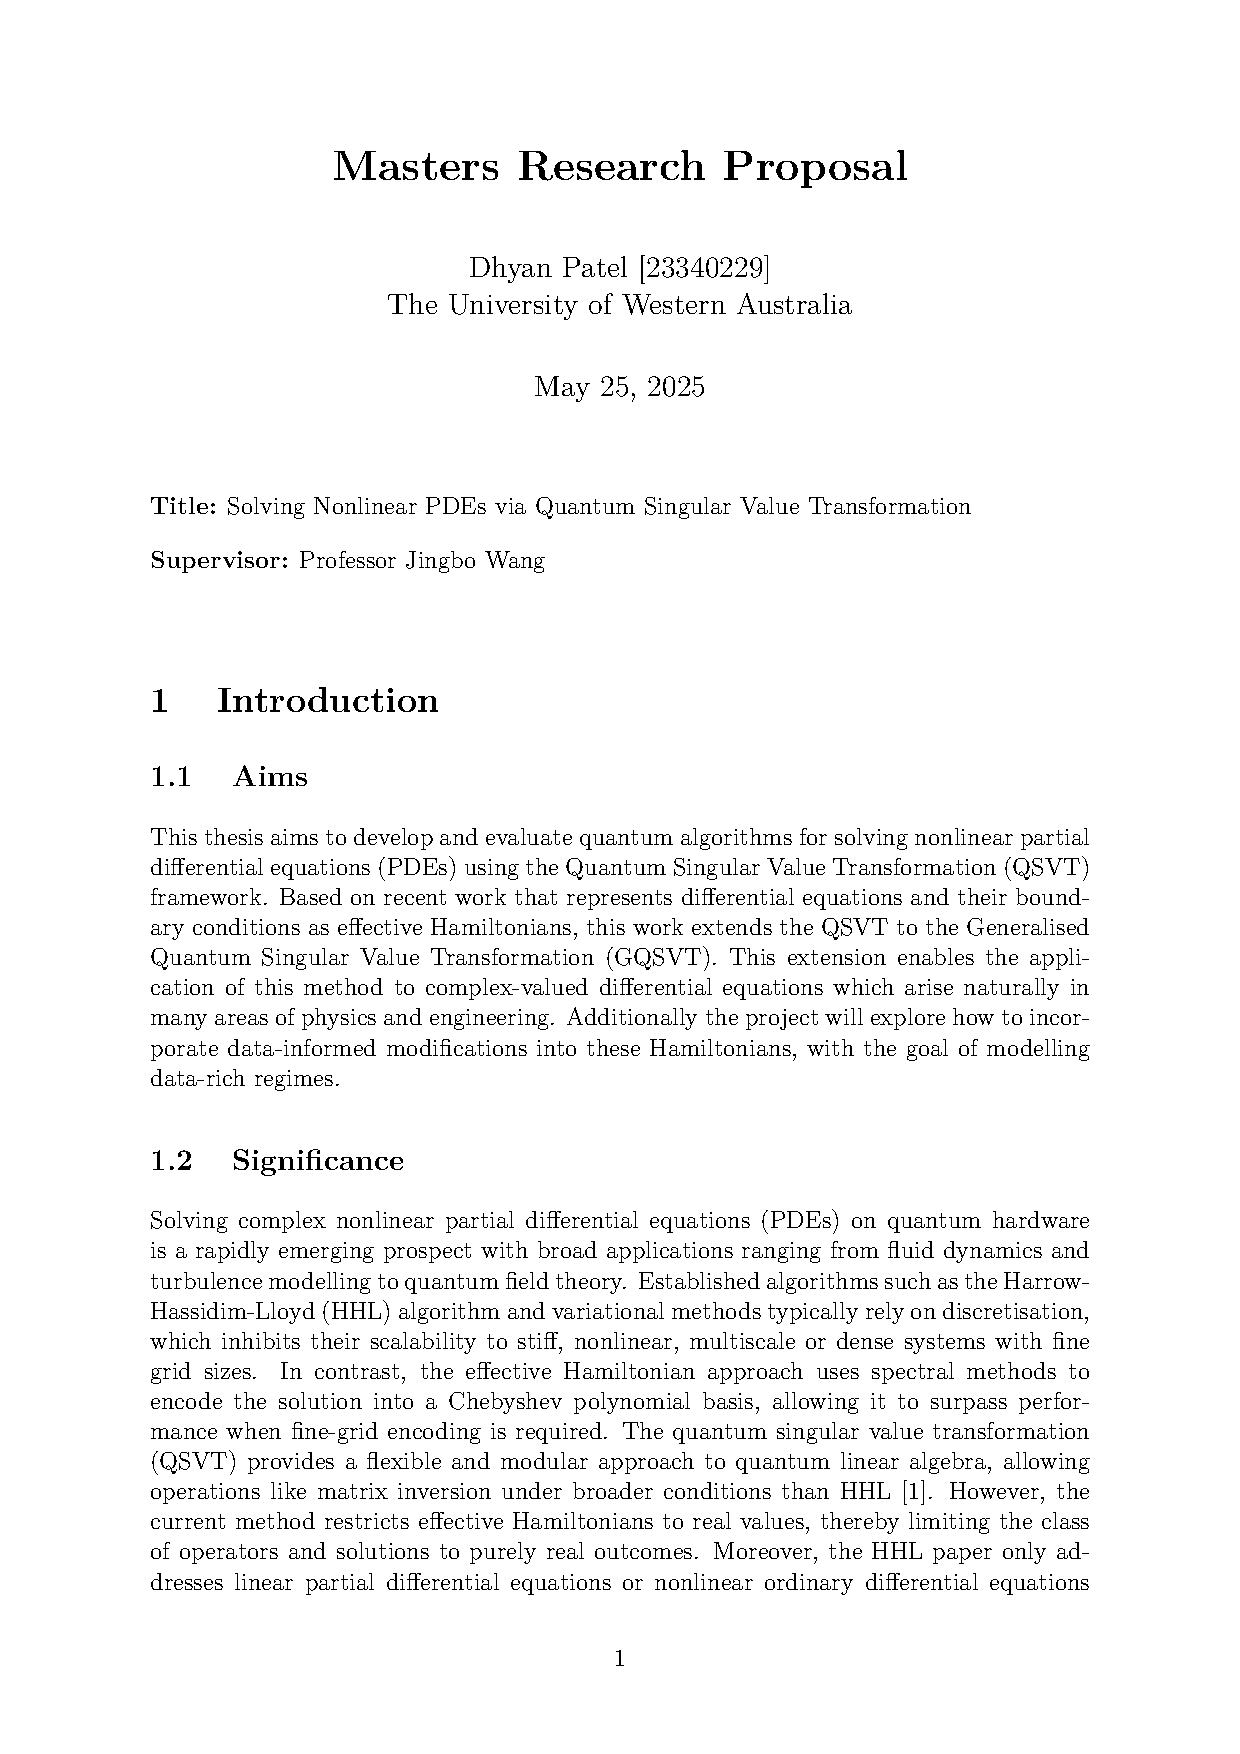
\includepdf[pages=-, scale=0.9, pagecommand={\thispagestyle{plain}}]{3_footer/research_proposal.pdf}
